\documentclass[14pt,landscape,color=UCLdarkred,margin=3cm]{uclposter}

\usepackage{amsmath,amssymb}
\usepackage{amsthm}
\usepackage{xcolor}
\usepackage{eso-pic}
\usepackage{authblk}
\usepackage{tikz}
\usepackage{environ}
\usepackage{graphicx}
\usepackage{float}
%\usepackage{physics}

\title{Scalable Quantum Simulation of Molecular Energies}

\author{James Mills}
\author{Shuhao Yang}
\author{Shanice St John}
\affil[1]{MSc Quantum Technologies, UCL}
% \affil[2]{TikZ, UCL}
% \affil[*]{a.example@ucl.ac.uk}

\begin{document}%\large

\maketitle

\begin{multicols}{3}

\section*{A new area for computing}


Quantum computing is a rapidly advancing field predicted to revolutionise many
areas of science and technology. It is predicted to have important applications in encryption and communication, and in the development of new medicines and materials. These quantum computers are not considered to be a replacement to classical (i.e. normal) computers, they will only be useful for certain types of problems which are too difficult for classical computers to solve. 

Simulating systems in quantum chemistry is too difficult for classical computers. Efficient simulation of quantum chemistry experiments would enable a dramatic leap forward in our understanding of fundamental chemistry. It would significantly reduce the need for cumbersome and expensive trial-and-error techniques in the development of new medicines and materials.

\section*{Key terms}


\begin{highlightbox}[UCLdarkblue!20!white]
	\textbf{Qubit} A quantum bit of information. Its classical counterpart, the bit represents classical information and is encoded in 0s and 1s. A qubit can be represented by a state.
\end{highlightbox}

\begin{highlightbox}[UCLstone!50!white]
  \textbf{Superposition} A qubit has extraordinary property, which can be in both states of `0' and `1' at the same time, but a classical bit is either `0' or `1'.
\end{highlightbox}



\begin{highlightbox}[UCLyellow!20!white]
\textbf{Quantum simulations in chemistry} Quantum theory is our best description of phenomena happening at the smallest scales imaginable. On a quantum computer, we are using quantum phenomena (the same phenomena that make the system difficult to describe with a classical computer) to precisely simulate chemistry structure and boost our computing power.
\end{highlightbox}

\begin{highlightbox}[UCLmidgreen!20!white]
\textbf{Algorithm} A set of instructions used to solve a problem, especially by a computer. The instructions are created so that it can be understood by the computer. This is then sent to the quantum computer. The computer then follows the instructions using some program or software. The end of the process provides an answer or even many possible answers.
\end{highlightbox}

\columnbreak

\section*{What are the techniques?}
The work by the researchers on the paper `Scalable Quantum Simulation of Molecular Energies' uses quantum qubits kept at very low temperatures to run algorithms to find out information about the fundamental properties of molecules.
The variational quantum eigensolver (VQE) and the phase estimation algorithm (PEA) are two types of algorithm which are performed on the qubit hardware to find molecular energies. A special type of quantum hardware known as Superconducting Quantum Interference Devices (SQUIDs) is used to run the algorithms. This type of qubit has a superposition of ``charged" states and can be used in quantum circuits.
\\
\begin{figure}[H]
  \begin{center}
%   \begin{minipage}[c]{15em}
\setlength{\fboxsep}{0.5em}
  \begin{minipage}[c]{9em}
  \begin{center}
  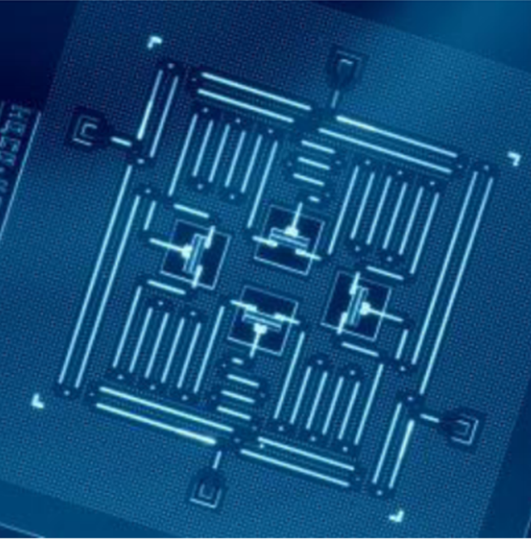
\includegraphics[width=7em]{4_Qubit.png}
    \caption{IBM qubit}
  \end{center}
    % 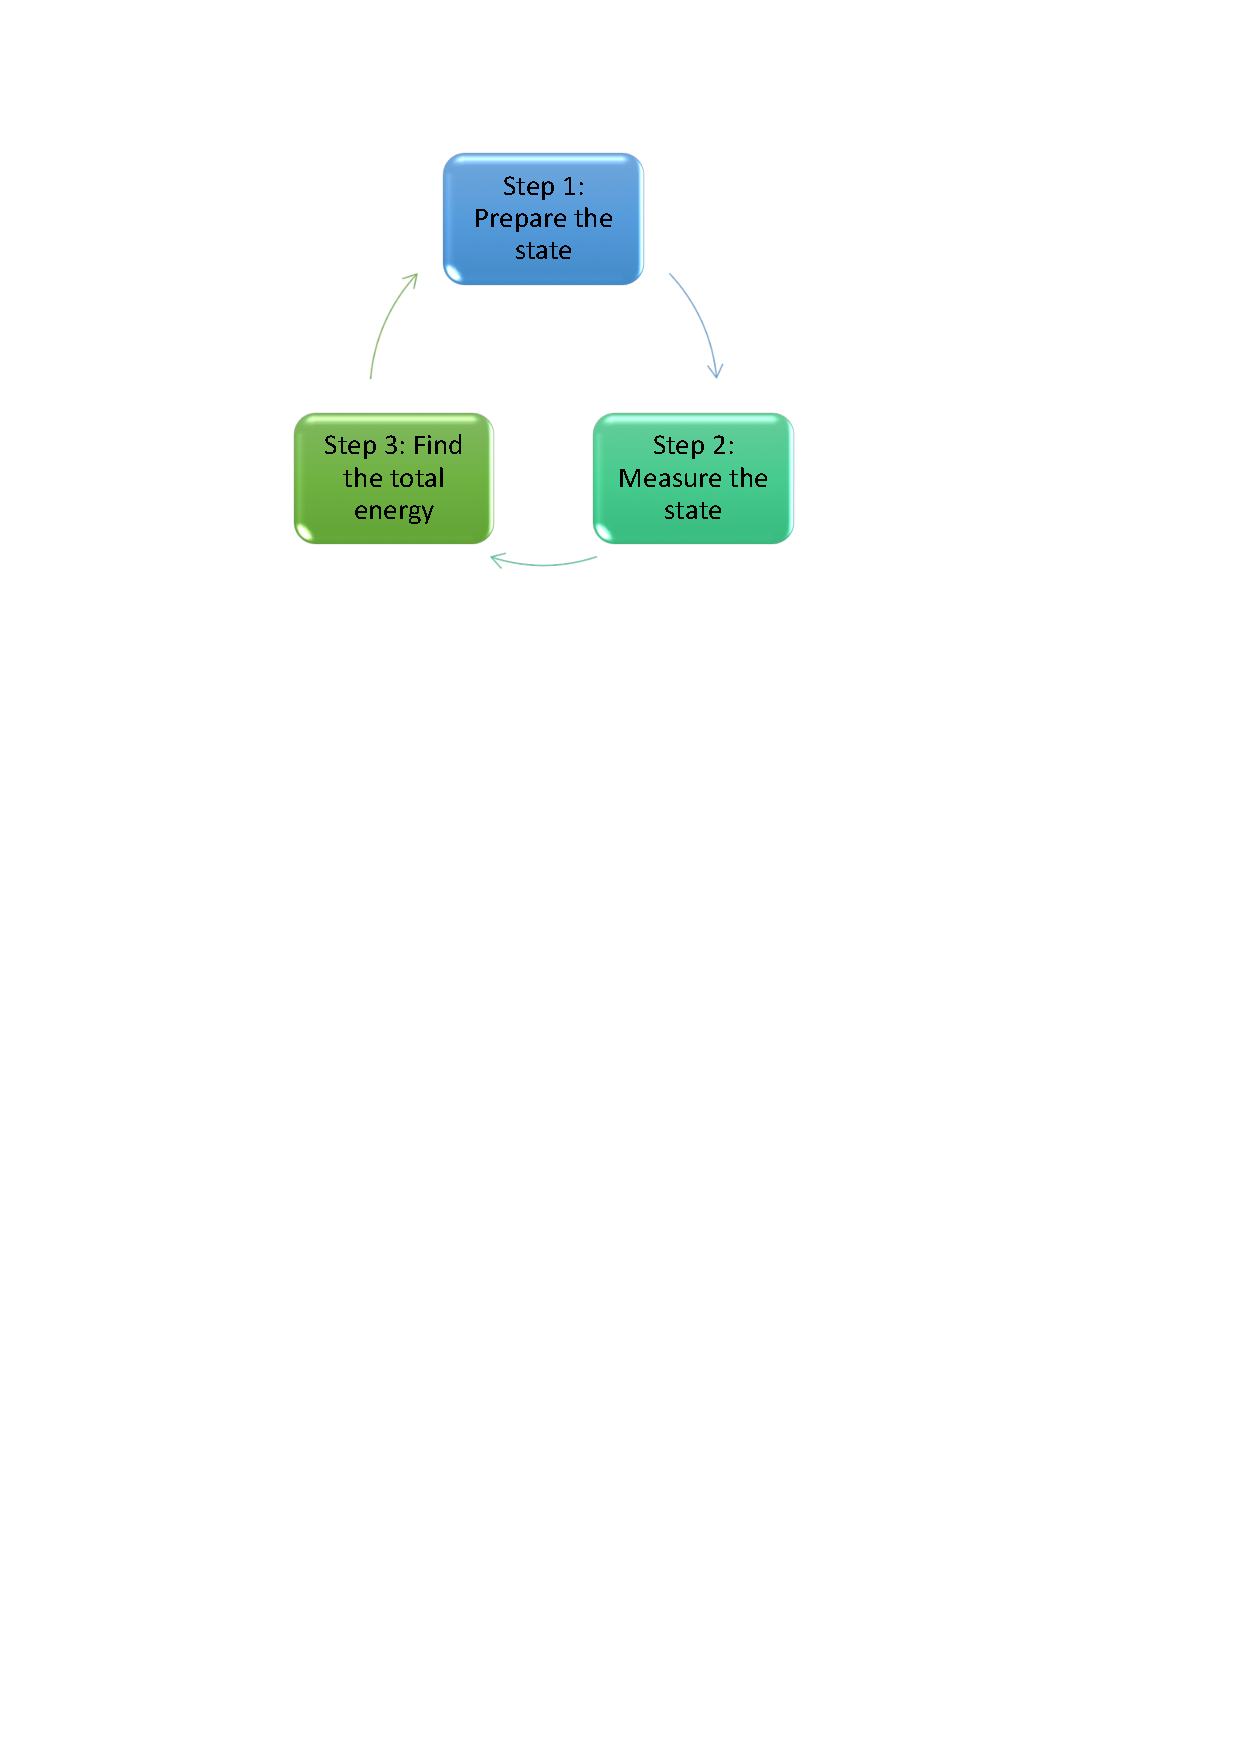
\includegraphics[width=15em]{VQEdiagram.pdf}
    
  \end{minipage}
  \qquad
  \begin{minipage}[c]{20em}
%   \begin{minipage}[c]{29em}
  %\large

The qubits used to run the algorithms were a type of charge qubit that is kept at very low temperatures like the IBM qubit.

  \end{minipage}
  \end{center}

   
\end{figure}

\section*{Algorithms for Quantum Chemistry}

The VQE algorithm uses the averages of the total energy so that the energy of a molecule can be calculated.

\begin{highlightbox}[UCLpink!20!white]
  \begin{enumerate}
\item We start by preparing a state using a ``special" method. This method makes it possible for the algorithm run in the way that we want.
\item Measure the total energy for each distance between the molecules. We must select the lowest value as we are focusing on the ground energy.
\item A tool is then used to find more lower values of the total energy.
\item Repeat until we reach the smallest value possible.
\end{enumerate}
\end{highlightbox}

PEA is the algorithm estimate the value of index over exponential coefficient in order to work out energy of a molecule.


\begin{highlightbox}[UCLpurple!20!white]
\begin{enumerate}
\item Similarly to the VQE algorithm, we must prepare a state using another ``special" method and encode information onto a exponential coefficient. 
\item Some equipment must be set up in a superposition of states - this will make it possible to measure the state.
\item We use operations to set up the state and the apparatus so that it is ready to be measured. 
\item Measure the state to find the lowest value of the total energy. We repeat this process until find an accurate value of the total energy.
\end{enumerate}
\end{highlightbox}



\begin{figure}[H]
  \begin{center}
   \begin{minipage}[c]{15em}
%  \begin{minipage}[c]{18em}
    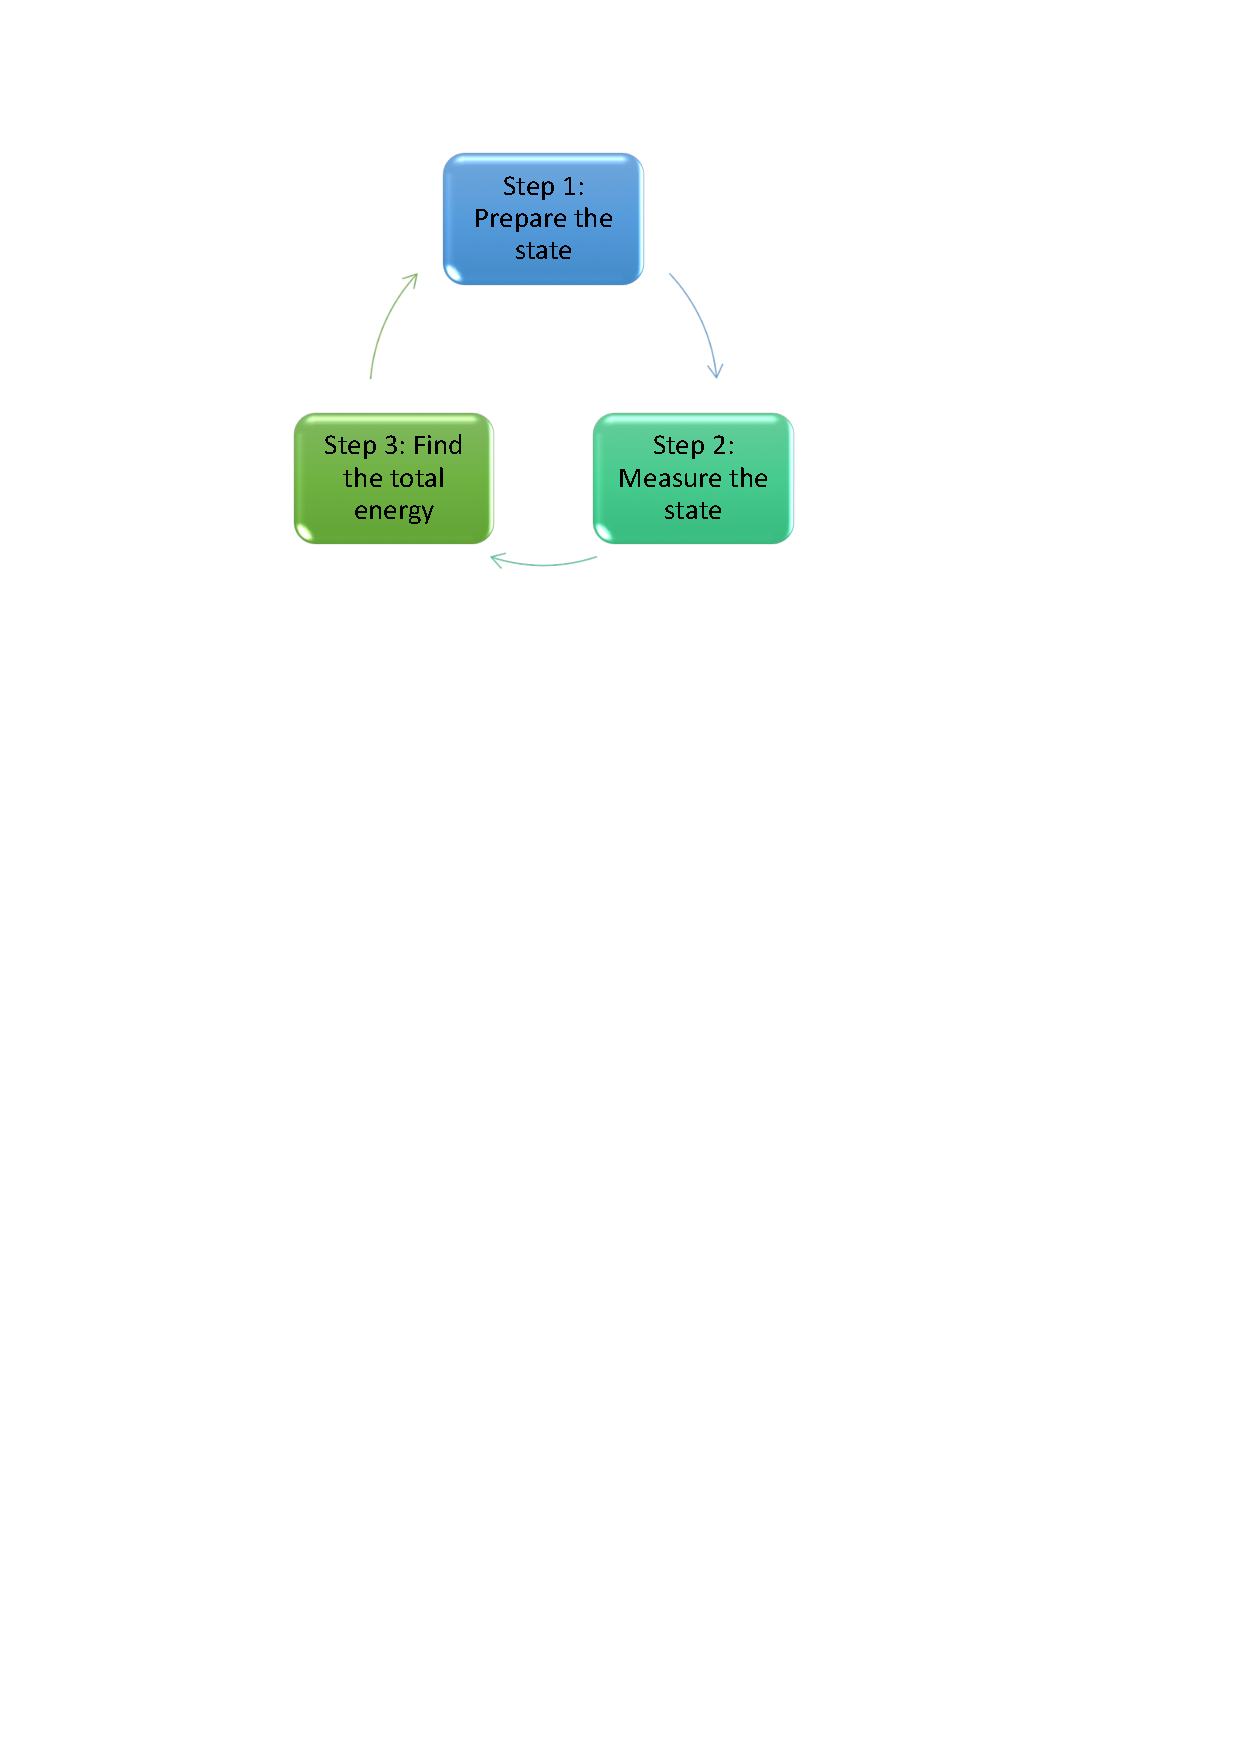
\includegraphics[width=15em]{VQEdiagram.pdf}
    % 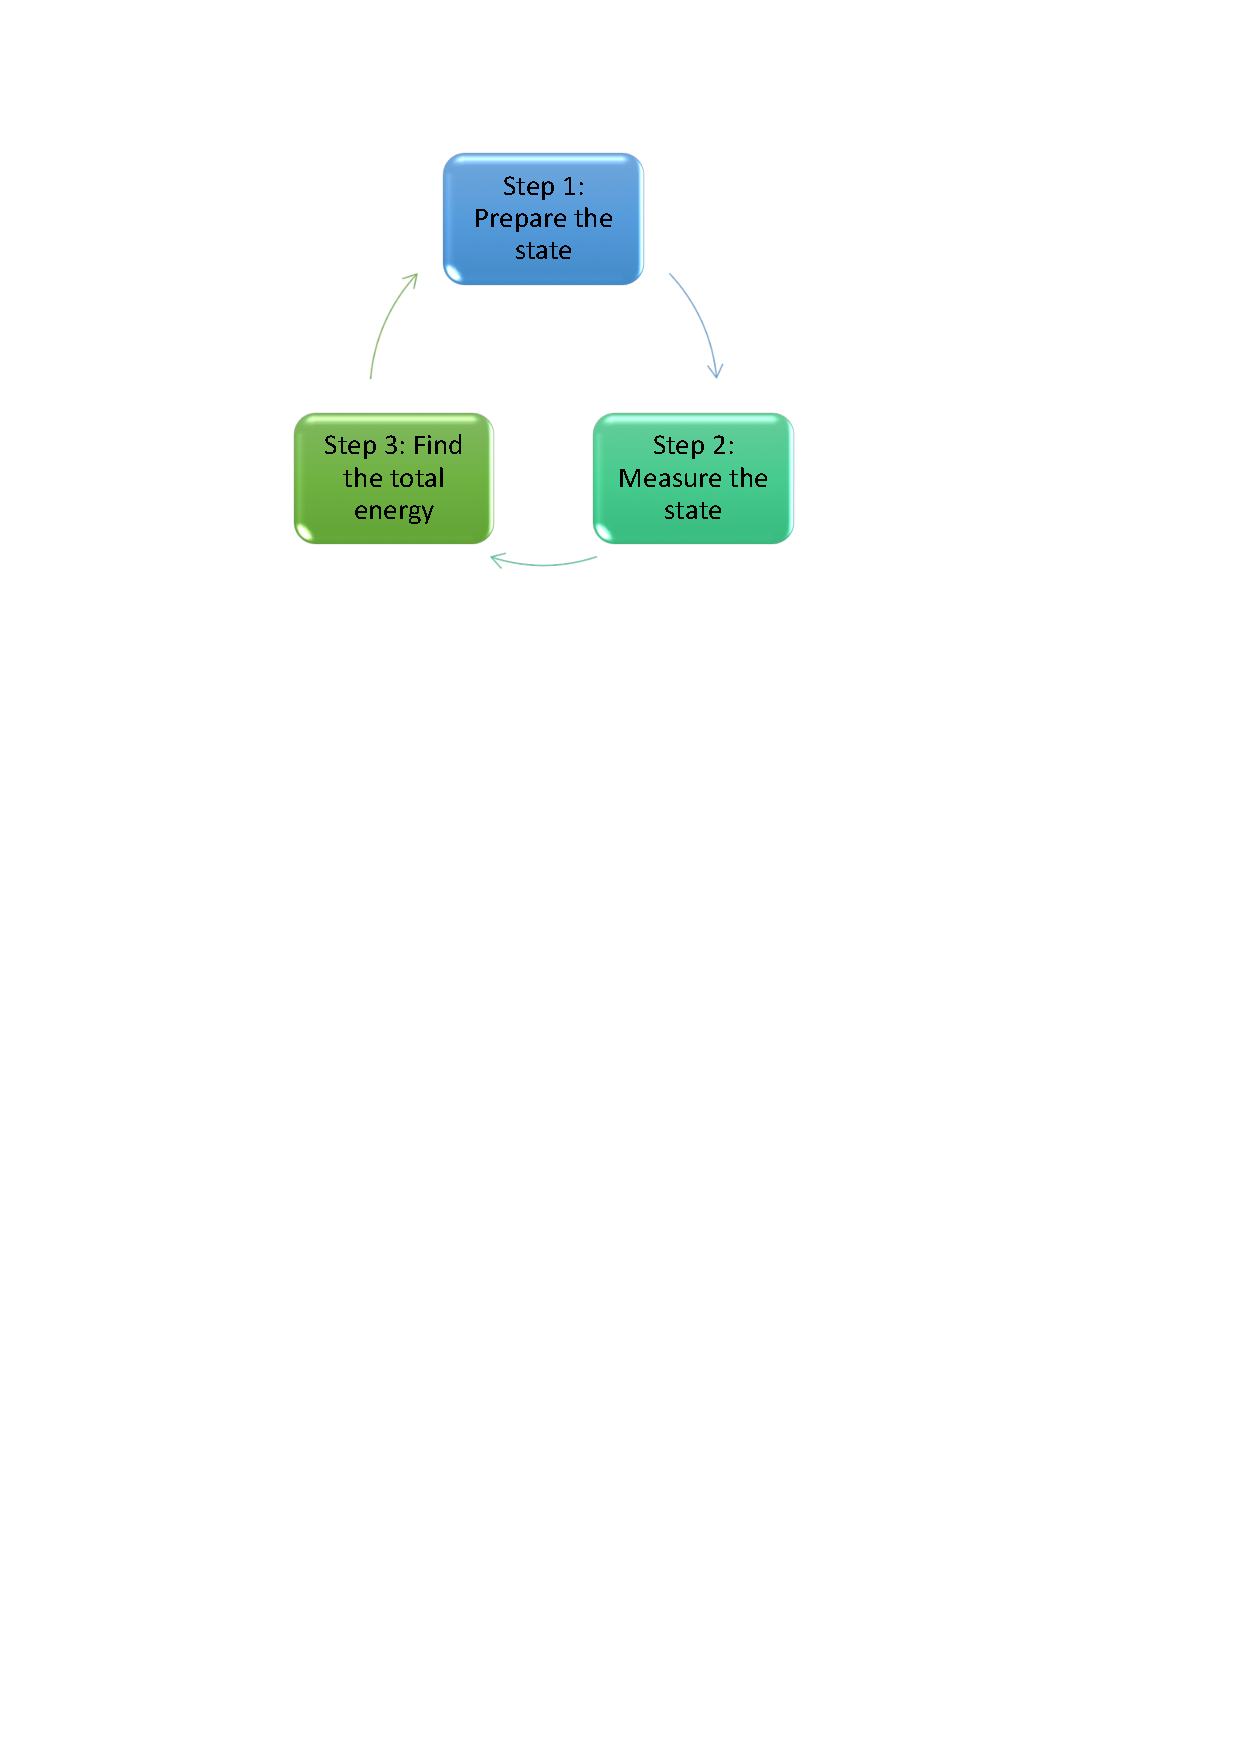
\includegraphics[width=18em]{VQEdiagram.pdf}
    \caption{VQE}
  \end{minipage}
  \qquad
  \begin{minipage}[c]{15em}
%   \begin{minipage}[c]{17em}
    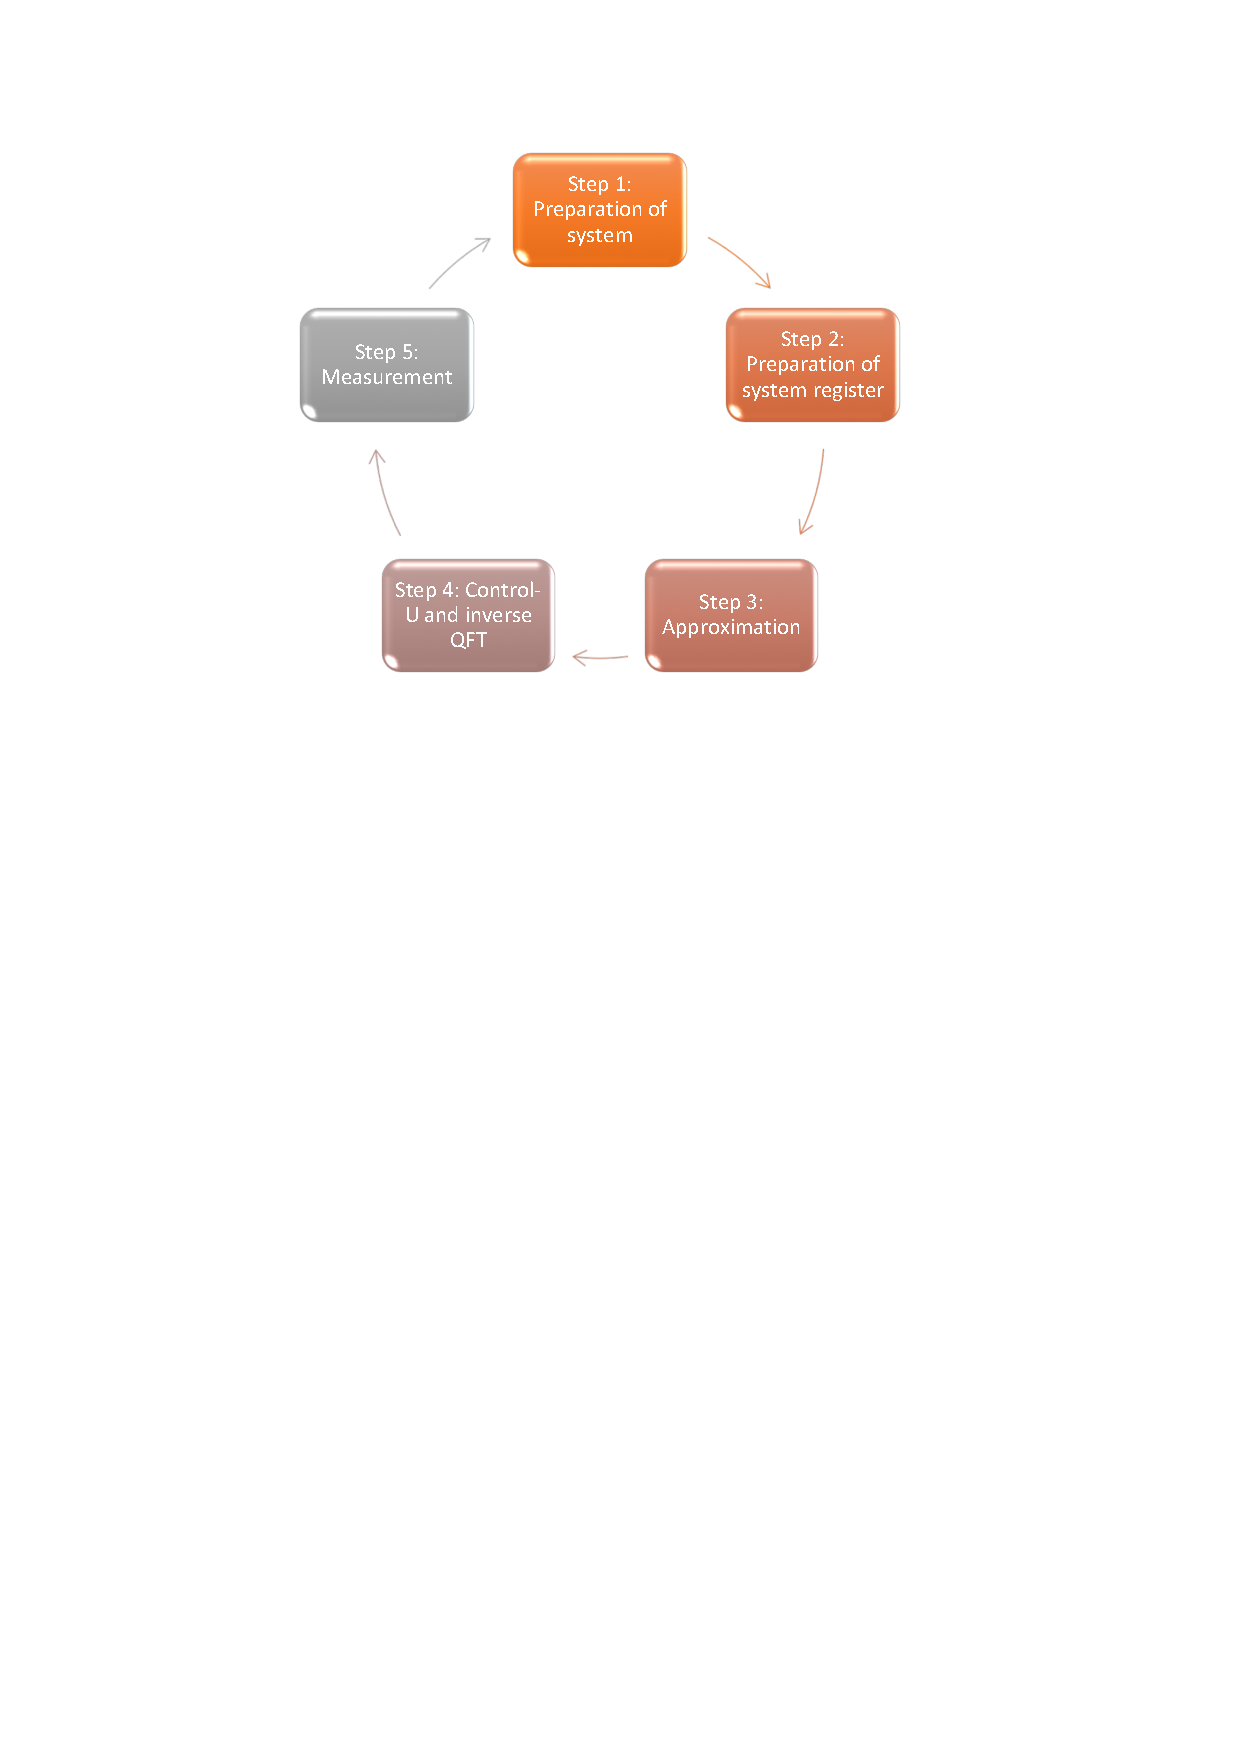
\includegraphics[width=15em]{PEA.pdf}
    % 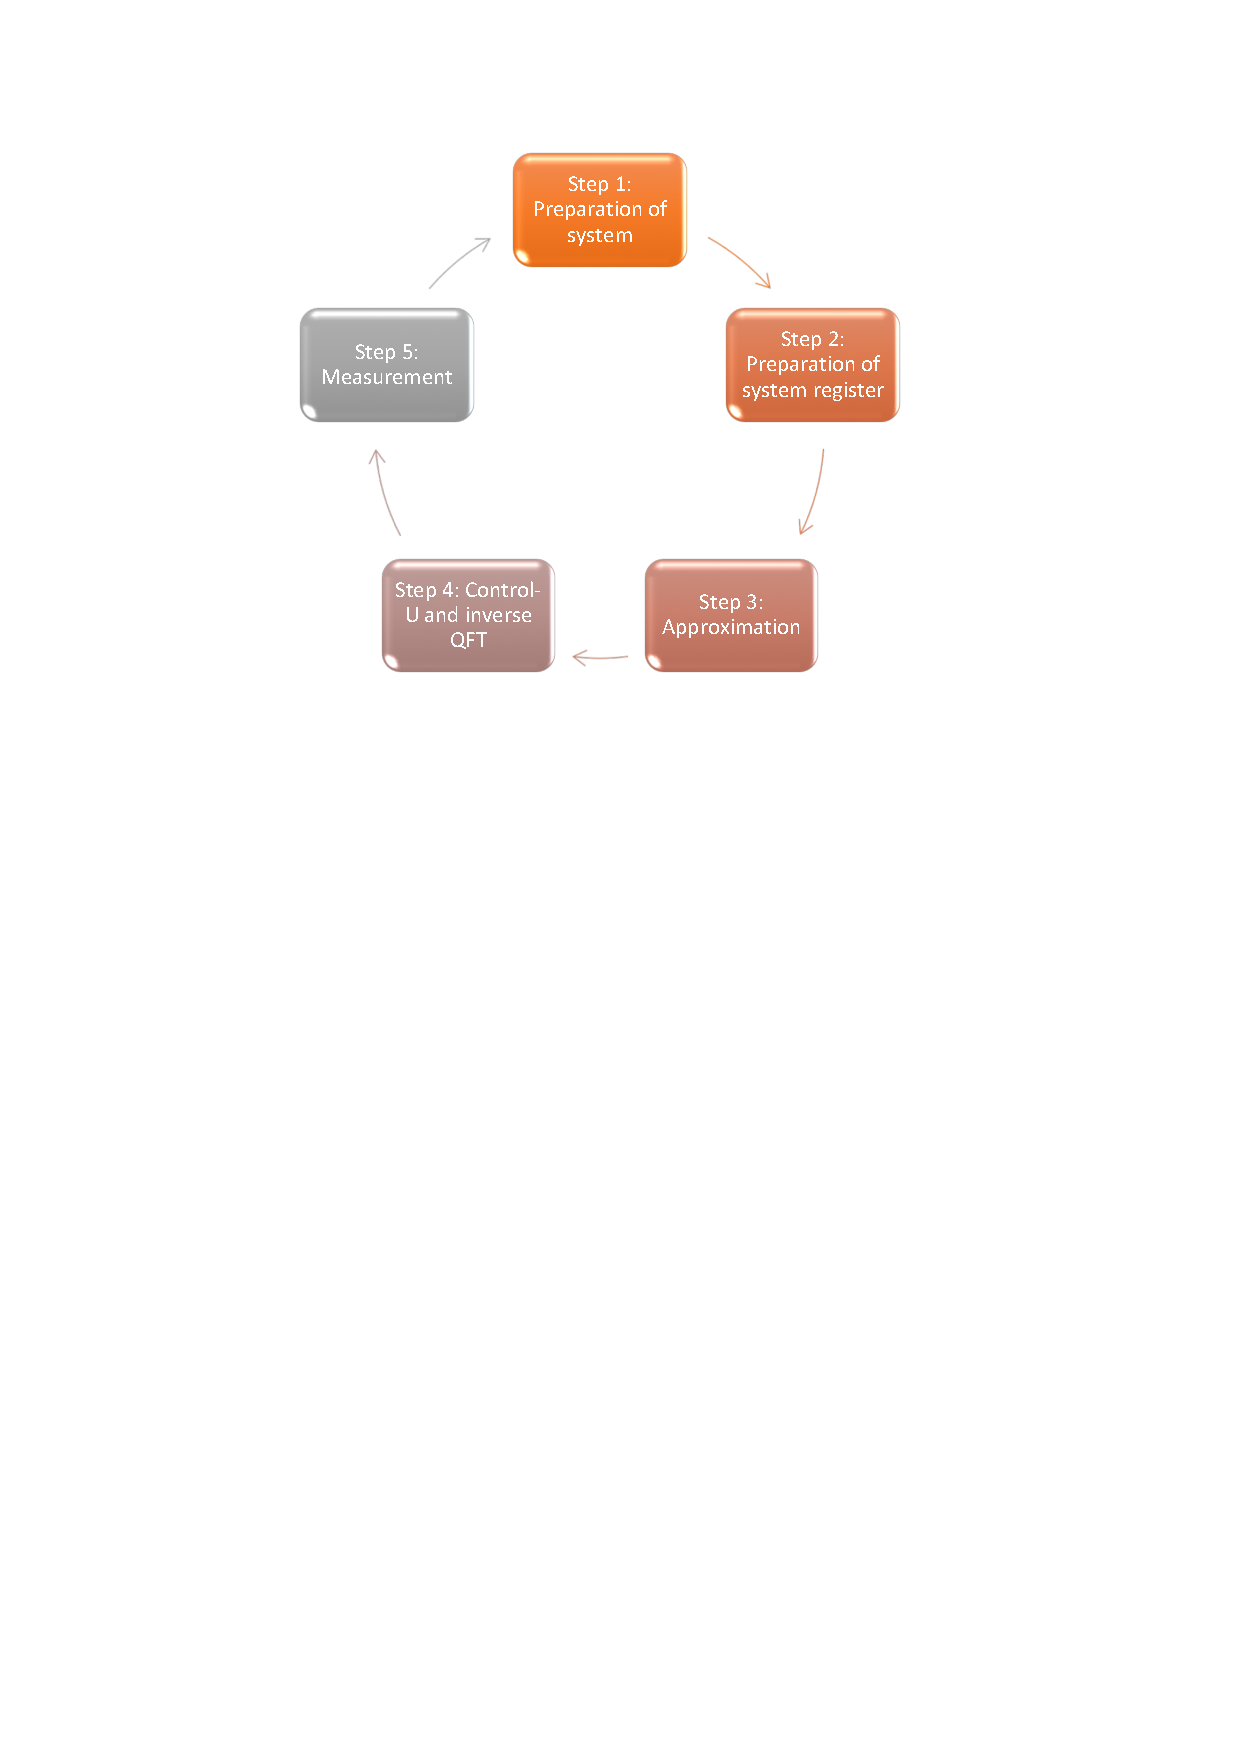
\includegraphics[width=17em]{PEA.pdf}
    \caption{PEA}
  \end{minipage}
  \end{center}

   
\end{figure}



\section*{Outlook}

The VQE was proven to work better than PEA because it gives more accurate results, this can be seen on Figure 4 where the VQE line is closer than the PEA line to the line representing the exact energy. This ability to simulate the quantum behaviour of atoms and molecules is hoped to offer new avenues for increasing our understanding of the world around us, and our ability to develop new medicines and materials!

\begin{figure}[H]
  \begin{center}
  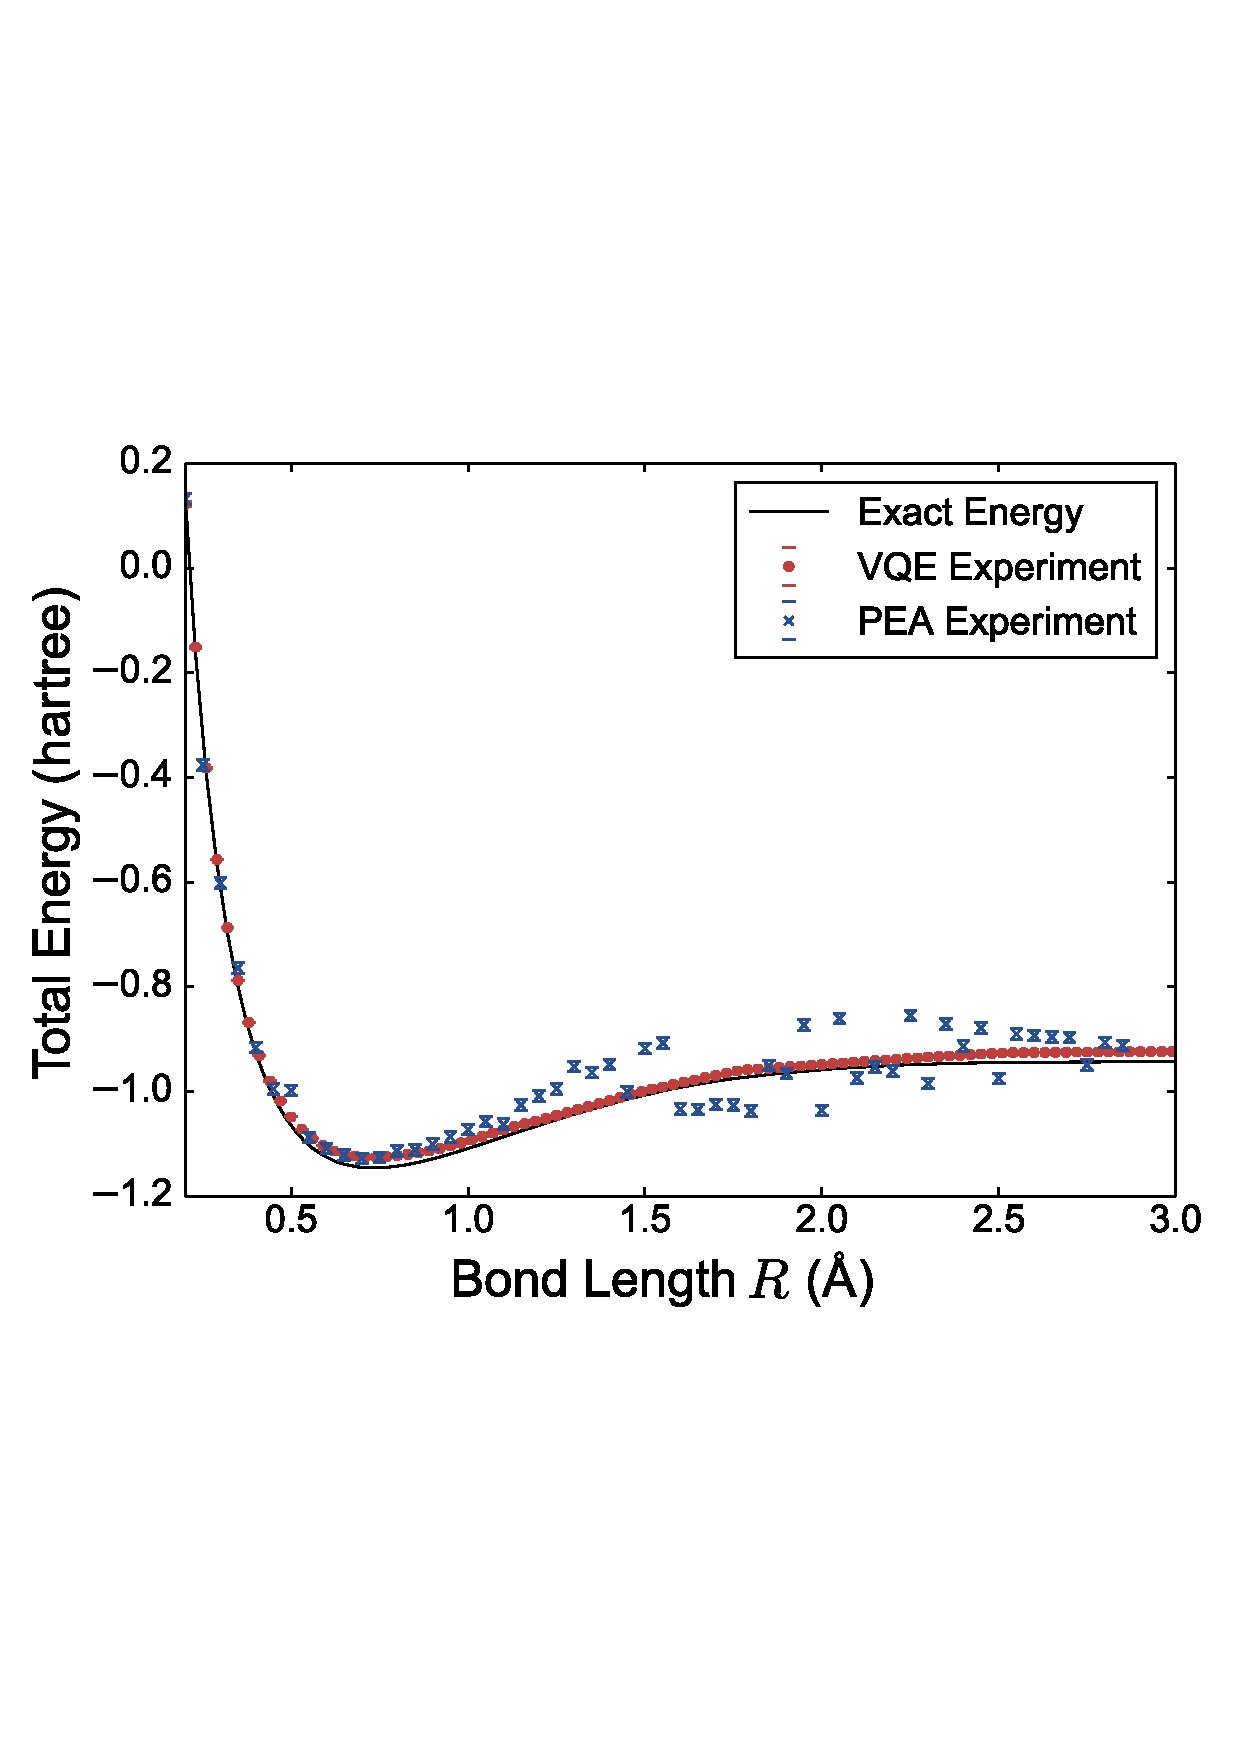
\includegraphics[scale=1.2]{result.pdf}
  \caption{Computed $H_2$ energy curve, energy surface of molecular hydrogen as determined by both VQE and PEA}
  \end{center}
    
 

   
\end{figure}



\end{multicols}
	
\end{document}
